\documentclass[sigconf]{acmart}
% Formatting from the competition's supplied Overleaf template.
\setcopyright{none}
\settopmatter{printacmref=false}
\acmConference[Kaggle Competition]{Filament Segmentation Challenge}{2026}{\href{https://www.kaggle.com/competitions/filament-segmentation-2026}{kaggle.com/competitions/filament-segmentation-2026}}
\acmBooktitle{Competition Report}
\acmDOI{}
\acmISBN{}
\usepackage{xcolor}
\newif\ifguideStyle
\guideStyletrue
\newcommand{\guide}[1]{\ifguideStyle{\color{gray!65}\itshape #1}\fi}
\usepackage{mathtools}
\usepackage{subcaption}
\usepackage{tabularx}
\usepackage{multirow}

\guideStylefalse
\begin{document}
\title{A Soft-Label ResNet U-Net Ensemble for Solar Filament Segmentation}
\subtitle{A Solution to the Solar Filament Segmentation Challenge 2026}
\author{Sijan Regmi}
\affiliation{\country{Nepal}}
\email{sijanregmi419@gmail.com}
\begin{abstract}
This report describes our solution to the Solar Filament Segmentation Challenge~2026, a Kaggle competition on automatic segmentation of solar filaments in GONG H-$\alpha$ observations. The final system averages the probability maps of two U-Nets with ImageNet-pretrained ResNet34 and ResNet50 encoders, trained at native $2048\times2048$ resolution on the mean of the annotators' masks (soft labels). Instead of one fixed threshold rule, instances are chosen from a tree of connected components built at thirteen thresholds: a gradient-boosted scorer, fitted on 111 calibration images, predicts each component's expected matched IoU, and an exact dynamic programme picks the disjoint set that maximizes expected PQ. All observations from one capture date stay in one data partition. On 139 held-out validation images this selection reaches micro Panoptic Quality (PQ) \textbf{0.4404} (date-cluster bootstrap 95\% interval [0.4188, 0.4598]), against 0.4271 for the fixed rule on the same probability maps and 0.1796 for our earlier classical baseline. The two submitted files use the networks trained on 457 images (public score \textbf{0.37}) and the same networks retrained on all 707 labelled images (public score \textbf{0.38}, no held-out score of its own). We release source code, notebooks, and checksums.
\end{abstract}
\maketitle
\section{Introduction}
This report goes over the details of our submitted solution to the Solar Filament Segmentation Challenge~2026 \cite{filament-segmentation-2026}. The challenge, launched on July~10,~2026, is organized by the Earth-Space AI Research (ESAIR) Lab\footnote{\href{https://www.esairlab.com/home}{www.esairlab.com/}}. This challenge utilizes the MAGFiLO dataset for evaluation of the segmentation algorithms \cite{ahmadzadeh2024dataset}.

Our first entry was a classical local-contrast pipeline (PQ 0.1796 on validation, 0.15 public). It misses weak filaments and confuses other dark features with filaments. We therefore replaced its pixel classifier by a supervised network and kept everything downstream unchanged: the date-grouped split, the metric, and the CSV format. This report describes that network system and, on top of it, a learned instance-selection step. The classical baseline remains in the repository for comparison.

\section{Methodology}\label{sec:methodology}
\subsection{Data, supervision, and external weights}
The archive contains 707 training images, 180 test images, and one annotation file with 1,154 annotator--image records (8,199 filament polygons). A source image has one, two, or three independent annotation sets (411, 145, and 151 images). Only the supplied segmentation polygons are used as supervision. Chirality labels, spines, bounding boxes, external images, and test labels are not used. The only external resource is the set of publicly available ImageNet-pretrained \texttt{torchvision} weights for ResNet34 and ResNet50 \cite{he2016resnet,torchvision}, free for every participant. The first convolution is reduced to one input channel by summing its three input-channel kernels.

\subsection{Data partitions and protocol}
Capture dates are assigned to partitions by a SHA-256 ordering within each year, so every image and annotator set from a date stays together. This gives 568 development images, of which 111 form the calibration subset, and 139 validation images. In every experiment the networks train on the 457 development images outside the calibration subset; checkpoints, post-processing, and the choice among candidates use calibration only, and validation is scored once per candidate. The final submission is the only exception: its networks are retrained on all 707 labelled images with settings fixed in advance (Section~\ref{sec:refit}).

\subsection{Network and training}
\begin{figure*}[t]
\centering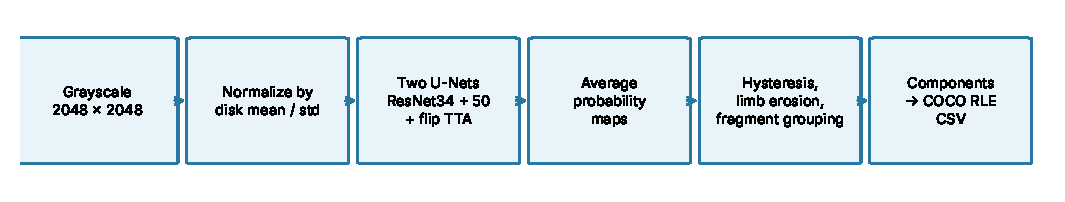
\includegraphics[width=\textwidth]{figures/gpu_pipeline.pdf}
\caption{Inference pipeline. Each test image is processed at native resolution by both networks with four flip views; the mean probability map is turned into instances by the post-processing of Section~\ref{sec:post}.}
\Description{Six-stage flow from grayscale image through normalization, two U-Nets, averaging, post-processing and CSV export.}
\end{figure*}
The network (\texttt{FilamentUNet}) is a U-Net \cite{ronneberger2015unet} whose encoder is a pretrained ResNet \cite{he2016resnet}. Because the ResNet stem halves the resolution at once and thin barbs are only a few pixels wide, a shallow two-layer branch at full input resolution is concatenated with the upsampled decoder output before a small prediction head. Input images are standardized with the mean and standard deviation of the solar disk.

The training target of an image is the mean of its annotators' masks. The metric scores a prediction against each annotator set separately, so this consensus is the best single probability map to aim for. The loss is binary cross-entropy plus soft Dice, both accepting soft targets. Training uses random $768\times768$ crops (70\% centred near an annotated pixel), dihedral flips, brightness and contrast jitter, and Gaussian noise. We use AdamW \cite{loshchilov2019adamw} with learning rate $5\cdot10^{-4}$, weight decay $10^{-4}$ and a one-cycle schedule \cite{smith2019onecycle}, 32 epochs of 150 steps with batch size 8, mixed precision, and an exponential moving average of the weights (decay 0.998) that is used for evaluation and inference. The ResNet34 and ResNet50 models use seeds 2027 and 2028. Inference runs on the full image and averages four flip views.

\subsection{Post-processing and instances}\label{sec:post}
The probability map is thresholded with hysteresis: pixels above a low threshold form regions, and a region is kept only if its peak reaches a high threshold. The solar disk is estimated per image by Otsu thresholding and eroded by 10 pixels to remove limb artifacts. Regions smaller than a minimum area are dropped. Fragments within about eight pixels of each other are merged into one filament, because ground-truth filaments are single polygons (none of the 8,199 contains several), while predictions often break up. Merging only labels fragments together; it adds no pixels. Each instance becomes one COCO run-length encoded row. The values were chosen by coordinate descent on calibration PQ over the grid in the repository: low threshold 0.6, high 0.9, minimum area 300, limb erosion 10, grouping distance 4 (hole filling off).

\subsection{Tree-based instance selection}\label{sec:tree}
The fixed rule above uses one threshold pair for every image. As an alternative, we build a component tree: the probability map (inside the eroded disk) is thresholded at 0.10, 0.15, \dots, 0.80, each connected component becomes a node, and a node's parent is the component that contains it at the previous level (components identical to their parent are merged). A node described by 31 features (area, shape, probability statistics, ring contrast, tree position) is scored by a histogram gradient-boosting regressor \cite{scikit-learn} trained to predict the node's expected matched IoU, that is, the mean over annotator sets of the IoU with a ground-truth filament when it exceeds 0.5. Because each prediction adds its expected IoU to the numerator of PQ and one half to the denominator, the expected-PQ-maximizing set of disjoint nodes is found exactly by dynamic programming on the tree, selecting nodes with score above a global cut-off $\tau$.

The scorer is trained on the 111 calibration images, using probability maps produced by networks that have not seen them. The scorer type (direct regression versus a hurdle model of match probability times IoU) and $\tau$ were chosen from out-of-fold scores on calibration, with folds by capture date: direct regression with $\tau=0.28$ (calibration out-of-fold PQ 0.4388, against 0.4368 for the hurdle model and 0.4240 for the fixed rule). The validation images were then scored once. For the final files, the scorer is refitted on calibration plus validation maps from the 457-image networks and applied to the test maps; for the 707-image networks the same scorer is applied to maps from networks that saw those images, a distribution shift we did not validate.

\subsection{Candidates, selection, and the refit}\label{sec:refit}
We compared five candidates (Table~\ref{tab:cand}) with the fixed rule and selected the two-network ensemble because it had the highest calibration PQ (0.4240); the tree-based selection of Section~\ref{sec:tree} was then added on top of that ensemble. The ResNet50 alone scored slightly higher on validation, but we did not choose by validation, because that would leak. For the submitted file we retrained the two networks, with identical settings and seeds, on training plus validation (707 images), kept the final EMA weights because no held-out images remain for checkpoint picking, and reused the post-processing tuned on calibration for the ensemble trained on 457 images. No parameter was re-tuned.

\section{Evaluation}\label{sec:evaluation}
\subsection{Metric}
Ground-truth polygons are rasterized with \texttt{pycocotools}. For each annotator--image record, a prediction and a ground-truth instance match when IoU $>0.5$; unmatched predictions are false positives and unmatched ground truths false negatives. Counts and matched IoUs are pooled over records, following the official self-evaluation notebook \cite{evaluation}:
\begin{equation}
\mathrm{PQ}=\frac{\sum_{(g,p):\mathrm{IoU}(g,p)>0.5}\mathrm{IoU}(g,p)}{\mathrm{TP}+0.5\mathrm{FP}+0.5\mathrm{FN}}.
\end{equation}
Uncertainty uses 2,000 bootstrap resamples of capture-date clusters (seed 2026). The interval reflects variation within this validation partition, not seed variance or unseen-date shift.

\subsection{Results}
\begin{table}[h]
\caption{Validation micro PQ (139 images, 222 annotator sets) of candidates trained on 457 images. ``Cal.'' is the calibration PQ used for selection (out-of-fold for the tree selection).}\label{tab:cand}
\centering\small\begin{tabular}{@{}lccc@{}}\toprule
Candidate & Cal. & Val. PQ & TP/FP/FN\\\midrule
Classical baseline & 0.176 & 0.1796 & 444/1160/1114\\
v1 U-Net, ResNet34, 512 px & -- & 0.4111 & 1047/813/511\\
ResNet34, 768 px, EMA & 0.417 & 0.4208 & 1015/674/543\\
ResNet50, 768 px, EMA & 0.420 & 0.4295 & 1020/644/538\\
Ensemble R34 + R50, fixed rule & 0.424 & 0.4271 & 1033/689/525\\
Ensemble R34 + R50, tree selection & 0.439 & \textbf{0.4404} & 937/401/621\\\bottomrule
\end{tabular}
\end{table}
All network candidates beat the baseline by a large margin, and their intervals overlap (Figure~\ref{fig:val}), so the differences among them are small relative to the uncertainty. The tree selection trades some true positives for far fewer false positives (689 to 401); its interval also overlaps the fixed rule's, but validation PQ is flat for $\tau$ between 0.20 and 0.34 (0.440 to 0.442), so the result does not depend on a fragile cut-off. A scorer with access to the true expected IoU of each node would reach 0.565 on validation, so the scorer, not the tree, is the limiting part. Instance grouping adds about 0.005 PQ. Two runs of the same v1 configuration differed by about 0.005 PQ (0.4060 and 0.4111) because GPU kernels are not bit-deterministic.

\begin{figure}[h]
\centering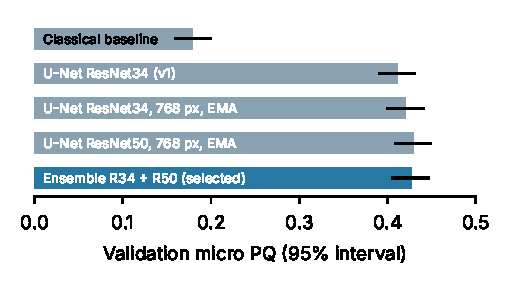
\includegraphics[width=\columnwidth]{figures/gpu_validation.pdf}
\caption{Validation PQ with 95\% date-cluster bootstrap intervals.}\label{fig:val}
\Description{Horizontal bars of validation PQ for five systems with interval whiskers.}
\end{figure}

\begin{table}[h]
\caption{Kaggle public leaderboard scores of the files we submitted for evaluation.}\label{tab:public}
\centering\small\begin{tabular}{@{}lc@{}}\toprule
Submission & Public score\\\midrule
Classical baseline & 0.15\\
v1 U-Net & 0.33\\
Ensemble trained on 457 images, fixed rule & 0.35\\
Ensemble refit on 707 images, fixed rule & 0.36\\
\textbf{457-image ensemble, tree selection (final)} & \textbf{0.37}\\
\textbf{707-image refit, tree selection (final)} & \textbf{0.38}\\\bottomrule
\end{tabular}
\end{table}
Public scores (Table~\ref{tab:public}) are about 0.07 to 0.08 below the local validation PQ, so we expect the private score to be lower than 0.4404 as well. On the same networks the tree selection scores 0.37 against 0.35 (457 images) and 0.38 against 0.36 (707 images) with the fixed rule, in line with the validation gain of +0.013. The refit has no held-out score; with the fixed rule it agreed closely with the 457-image ensemble on the test images (matched PQ 0.884, mean pixel Dice 0.956). Kaggle shows only two decimals and the public part is about half of 180 test images, so differences of 0.01 do not prove that the extra data or the tree selection helps; the validation gain and the public gains point the same way.

\subsection{Error analysis and limitations}
Annotators disagree strongly under this metric: scoring one annotator's filaments against another's gives PQ 0.353 on the 101 images with two or more annotators. Our predictions exceed that because they target the annotators' consensus. The consensus mask itself reaches PQ 0.78 on calibration, which is an optimistic upper reference because single-annotator images are scored against their own mask. On validation, false positives (689) outnumber false negatives (525). The system is selected on one split, one seed per network and one calibration subset. Models are trained on a single archive of GONG images, so other instruments or epochs are untested. A larger grouping distance hurts: the consensus mask drops from PQ 0.78 to 0.68 at 32 pixels.

\subsection{Reproduction}
\sloppy
Code is in the public repository; \path{notebooks/gpu-experiments-v2.ipynb} reproduces the candidate comparison and \path{notebooks/gpu-refit-707.ipynb} the 707-image networks on a Kaggle T4$\times$2 (about 2.8~h and 1.4~h); \path{notebooks/gpu-treesel.ipynb} regenerates the probability maps from those saved networks and runs the tree selection (about 23~min). The two files selected on Kaggle are \path{treesel/submission_refit_models.csv} (public 0.38; 1,155 rows, 180 test images, 177 with predictions; SHA-256 prefix \texttt{2a01f6e0}) and \path{treesel/submission_held_out_models.csv} (public 0.37; 1,131 rows, 177 images with predictions; SHA-256 prefix \texttt{8c900861}), both verified for column format, unique identifiers, and canonical RLE; full digests are in the repository. Trained weights are not stored in git; they are recreated by the notebooks, and the tree notebook reads the models and the fixed-rule baseline from the recorded candidate-comparison and refit runs. The classical code is unchanged. AI assistance was used to develop and document the code; the participant must independently understand and defend its operation under the competition rules.

\balance
\section{Acknowledgment}\label{sec:acknowledgment}
The organization of the Filament Segmentation Challenge 2026 is partially supported by the U.S. National Science Foundation (NSF) under Grant No. 2209912 and 2433781, directorate for Computer and Information Science and Engineering (CSE), and Office of Advanced Cyberinfrastructure (OAC), and Grant No. 2511630, AST Division Of Astronomical Sciences and MPS Directorate for Mathematical and Physical Sciences.

The Filament Segmentation Challenge 2026 is sponsored by the U.S. National Science Foundation (NSF) National Solar Observatory (NSO).

This work utilizes GONG data obtained by the NSO Integrated Synoptic Program, managed by the National Solar Observatory, which is operated by the Association of Universities for Research in Astronomy (AURA), Inc. under a cooperative agreement with the National Science Foundation and with contribution from the National Oceanic and Atmospheric Administration. The GONG network of instruments is hosted by the Big Bear Solar Observatory, High Altitude Observatory, Learmonth Solar Observatory, Udaipur Solar Observatory, Instituto de Astrofísica de Canarias, and Cerro Tololo Interamerican Observatory.
\bibliographystyle{ACM-Reference-Format}
\bibliography{main,gpu}
\end{document}
